% Part 2 chapter carrying "The Cosmological Constant as Actualized Vacuum Energy" (March 2026), sections 7-10, line for line
% (PDF read in full 2026-10-03, 842 lines), with the history integral that "Matter-Antimatter Asymmetry and the Information Writing
% Constraint" section 3 shares (given once, here). Corrections: PAPER_ERRATA C2, C16, C18, C22; CC_AND_BARYON_CHECK.md items 3-4,
% 16-17 and the accumulation test. Numbers: docs/verification/scripts/verify_lambda_baryon_book.py, sections A, C;
% the accumulation test from verify_cc_and_baryon.py section 6. Figure: figscripts/fig_p2_lambda_history.py.
\chapter{The cosmological constant over cosmic history}\label{ch:lambda_history}

Chapter~\ref{ch:lambda} evaluated the cosmological-constant expression with today's values of $\Omega_b/\Omega_m$ and $l_H$. If
$\Lambda$ is an accumulated cost, it has a history: it grows as baryonic decoherence writes more of the horizon, and its value today is
an integral over the epochs since the matter sector began. This chapter carries that history --- the growth of $\Lambda$ with time, the
history integral, and a direct test of what the accumulated quantity can be --- and closes with the place of the reading among other
approaches and its conclusions.

\section{The cosmological constant is not constant}\label{sec:lh_notconst}
A direct consequence of reading $\Lambda$ as an accumulated cost is that the cosmological ``constant'' is not strictly constant.
The accumulated Landauer cost grows as the universe ages and more baryonic decoherence events write information onto the horizon. The
accumulation is governed by the activation function $E(a)=\exp(1-1/a)$ (Chapter~\ref{ch:theory}), which increases monotonically. As
$E(a)$ advances, the accumulated cost increases, and $\Lambda$ increases slowly with cosmic time. \conjecture

The rate of increase today follows from
\begin{equation}\frac{dE}{da}=\frac{E(a)}{a^2},\qquad \frac{dE}{da}\Big|_{a=1}=1 .\label{eq:lh_dE}\end{equation}
\derived\ A component whose density grows with the scale factor has, from the continuity equation $\dot\rho+3H(\rho+P)=0$ with
$P=w\rho$,
\begin{equation}w=-1-\frac13\frac{d\ln\rho}{d\ln a}.\label{eq:lh_w}\end{equation}
\derived\ A growing density, $d\ln\rho/d\ln a>0$, therefore has $w<-1$. Writing the equation of state as
\begin{equation}w=-1-\epsilon(a),\qquad \epsilon(a)=\frac13\frac{d\ln\rho}{d\ln a}>0,\label{eq:lh_eps}\end{equation}
the dark-energy equation of state of an accumulating $\Lambda$ lies below $-1$. For a contribution proportional to $E(a)$,
$d\ln\rho/d\ln a=a\,E'/E=1/a$, so
\begin{equation}w_{\rm info}(a)=-1-\frac{1}{3a},\qquad w_{\rm info}(1)=-\frac43,\label{eq:lh_winfo}\end{equation}
the equation of state of the structural term derived in Chapter~\ref{ch:theory}. \derived\ It is further below $-1$ at earlier epochs,
when the term itself is small. The combined dark sector --- the vacuum baseline with $w=-1$ plus the growing term --- has an effective
equation of state between the two (Chapter~\ref{ch:theory}, Chapter~\ref{ch:darkenergy}). \calc

DESI DR2 reports a 2.8--4.2$\sigma$ preference for dynamical dark energy, with $w_0>-1$ today and $w_a<0$~\cite{DESI2025}. \observed\ An
accumulating $\Lambda$ gives $w<-1$ for the growing part, so the direct sign comparison with the DESI $w_0$ does not hold; whether the
combined dark sector, read through the CPL parametrisation DESI uses, is consistent with the DESI posterior is the comparison of
Chapters~\ref{ch:sectortension} and~\ref{ch:darkenergy}, and it is open. \openprob\ The growth of $\Lambda$ follows from the activation
function, which was derived from horizon thermodynamics (Chapter~\ref{ch:theory}) independently of the DESI results; it was not added to
accommodate them.

\section{The full decoherence history integral}\label{sec:lh_integral}
The calculation of Chapter~\ref{ch:lambda} uses today's values of $\Omega_b/\Omega_m$ and $l_H$. A fuller treatment integrates the
baryonic decoherence contribution over the cosmic history, from the onset of the matter sector at electroweak symmetry breaking
(Chapter~\ref{ch:electroweak}) to today ($a=1$). The accumulated cosmological constant at scale factor $a$ is written
\begin{equation}
\frac{\Lambda(a)}{\rho_{\rm vac}}\propto\int_{a_{\rm EW}}^{a}\frac{\Omega_b(a')/\Omega_{\rm tot}(a')}{l_H(a')^2/l_P^2}\,
\frac{da'}{a'^2H(a')/H_0},\label{eq:lh_integral}
\end{equation}
where $\Omega_b(a')/\Omega_{\rm tot}(a')$ is the baryonic fraction of the total energy density at scale factor $a'$ and
$l_H(a')=c/H(a')$ is the Hubble length at that epoch. \conjecture\ The integrand is the writing rate per unit scale factor: the fraction
of the horizon's Planck-area bits being written by baryonic decoherence at each epoch, weighted by the baryonic fraction of the energy
and by the inverse square of the Hubble length.

The intention was that the integral weights each epoch correctly: during radiation domination ($a\ll a_{\rm eq}$) baryons are a small
fraction of the total energy; during matter domination they are a larger fraction; during dark-energy domination the Hubble length
approaches its present value. The integral does not do this. With $(l_P/l_H(a'))^2=(l_P/l_H)^2[H(a')/H_0]^2$, the integrand is
$(l_P/l_H)^2\,[\Omega_b(a')/\Omega_{\rm tot}(a')]\,[H(a')/H_0]/a'^2$. In the radiation era $\Omega_b/\Omega_{\rm tot}\propto a'$ and
$H\propto a'^{-2}$, so the integrand grows as $a'^{-3}$ toward early times and the integral is set by its lower limit. \derived\
Evaluated from the printed $a_{\rm EW}=2.3\times10^{-15}$, with Planck 2018 densities and radiation $\Omega_r=9.22\times10^{-5}$, and written
as a coefficient $K$ in $K(l_P/l_H)^2\,\Omega_b/\Omega_m$, it gives
\begin{equation}K_{\rm integral}=3.1\times10^{30}\qquad\text{against the required}\qquad K=\frac{3\Omega_\Lambda/8\pi}{\Omega_b/\Omega_m}=0.523 .
\label{eq:lh_K}\end{equation}
\calc\ The scale factor at a temperature of 100\,GeV with entropy conservation ($g_{*s}=106.75$) is $7.8\times10^{-16}$, not
$2.3\times10^{-15}$, which raises $K_{\rm integral}$ to $2.7\times10^{31}$; at the crossover temperature 159.5\,GeV
(Chapter~\ref{ch:electroweak}) it is $6.9\times10^{31}$. Starting the integral later only lowers the excess: $6.5\times10^6$ from
$a=10^{-3}$. \calc\ The dominant contribution therefore comes from the earliest epoch, not the late-time, dark-energy-dominated one, and
the integral as written gives neither the $\sqrt{\Omega_\Lambda}$ factor nor the coefficient. Its normalization and evaluation are
open. \openprob

\begin{figure}[htbp]\centering
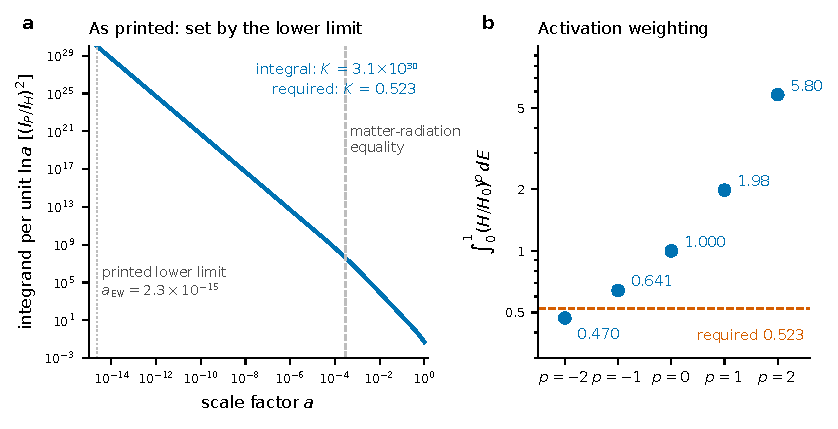
\includegraphics[width=\textwidth]{figures/part2/fig_cc_history.pdf}
\caption[The history integral and the activation weighting]{(a) The integrand of Eq.~\eqref{eq:lh_integral} per unit $\ln a$ (in units of $(l_P/l_H)^2$), from the printed lower limit $a_{\rm EW}=2.3\times10^{-15}$ to today: it falls as $a^{-2}$ per $\ln a$ through radiation domination, so the earliest epoch dominates and the integral gives $K=3.1\times10^{30}$ against the required $0.523$. (b) The same quantity weighted by the growth of the activation, $\int(H/H_0)^p\,dE$, for $p=-2,\dots,2$, on the 18th-chain $\Omega_m=0.3198$: $0.470$, $0.641$, $1$, $1.983$, $5.797$, against the required $0.523$ (dashed). None is selected by a derivation. Planck 2018 densities~\cite{Planck2018VI}; \texttt{verify\_lambda\_baryon\_book.py}, section C. \calc\ \openprob}\label{fig:cc_history}
\end{figure}

Weighting the same quantity by the growth of the activation, $dE(a)$, instead of $da/a^2$, removes the divergence and gives O(1)
coefficients, but which one depends on the form chosen. On the 18th-chain $\Omega_m=0.3198$:
\begin{equation}\begin{gathered}
\int_0^1\!\Big(\frac{H_0}{H}\Big)^2dE=0.470,\quad \int_0^1\!\frac{H_0}{H}\,dE=0.641,\quad \int_0^1\!dE=1,\quad
\\ \int_0^1\!\frac{H}{H_0}\,dE=1.983,\quad \int_0^1\!\Big(\frac{H}{H_0}\Big)^2dE=5.797 .
\end{gathered}\label{eq:lh_weights}\end{equation}
\calc\ None is selected by a derivation; choosing the closest ($0.470$, 10\,\% below $0.523$) after seeing the target would be a fit.
The history integral has to be written in the variable that carries the cost, which the next section identifies.

\section{What the accumulated quantity is}\label{sec:lh_accum}
A direct test, with no free factors, asks whether the accumulated quantity could be the heat that baryons radiate as they virialise.
Take the halo mass function of Sheth and Tormen~\cite{ShethTormen1999} above $10^8\,M_\odot$, with an Eisenstein--Hu power
spectrum~\cite{EisensteinHu1998} normalised to $\sigma_8=0.811$, and the virial kinetic energy per unit mass of a uniform sphere,
$\tfrac{3}{10}GM/r_{\rm vir}$. By the virial theorem the heat radiated in virialisation equals the kinetic energy stored. Summed over all
baryons in halos today:
\begin{itemize}
\item the baryon mass fraction in halos is $0.58$, with a mean dispersion $\sigma_{\rm eff}=213$\,km\,s$^{-1}$; \calc
\item the accumulated virial heat of baryons is $3.1\times10^{-8}\,\rho_\Lambda c^2$; \calc
\item priced at the horizon (bits $=Q/(k_BT_{\rm gas}\ln2)$, each costing $k_BT_{GH}\ln2$) it is $2.6\times10^{-44}\,\rho_\Lambda c^2$; \calc
\item the upper bound, all baryon rest mass converted, is $\Omega_b/\Omega_\Lambda=0.072$ of $\rho_\Lambda$. \calc
\end{itemize}
Heat radiated by baryons is $3\times10^{-8}$ of $\rho_\Lambda c^2$, so radiated heat is not the measure of the accumulated cost. The
informational term's size is set by the virial partition of the matter itself, $\beta_m=\Omega_m/2$ (the kinetic half), activated by
$E(a)$: a horizon-entropy term in the first law, priced by IAM's Law at $k_BT_{GH}\ln2$ per bit on the horizon. \interp\ The history
integral of Section~\ref{sec:lh_integral} must be written in that variable. \openprob\ In this picture $\Lambda$ is the vacuum baseline
before structure and accumulates as structure forms and decoherence accelerates; the baseline and the accumulated value are the same
picture at two epochs. \interp

\section{Relation to other approaches}\label{sec:lh_prior}
The cosmological constant problem has been approached from several directions. Weinberg~\cite{Weinberg1989} gave an anthropic bound on
$\Lambda$ but not a derivation of its value. Supersymmetric cancellations reduce the discrepancy by some orders of magnitude but do not
remove it~\cite{Witten2001}. The string landscape~\cite{BoussoPolchinski2000} provides a framework for anthropic selection but does
not give $\Lambda$ from first principles. Unimodular gravity~\cite{Weinberg1989} reformulates the problem without resolving it.

The approach carried here differs in two respects. It does not try to reduce the theoretical vacuum energy: the Planck-scale vacuum
energy density is taken as the correct total quantum capacity. And it invokes no selection mechanism or anthropic argument: the observed
$\Lambda$ is read as a consequence of the universe's decoherence history, computed from physical constants and measured cosmological
parameters. \interp\ The O(1) prefactors of that computation are taken as given here; their derivation is an open problem (Chapter~\ref{ch:lambda}). \openprob

The closest approaches in spirit are Verlinde's entropic gravity~\cite{Verlinde2011} and Padmanabhan's thermodynamic reading of
gravity~\cite{Padmanabhan2010}, both of which connect gravitational physics to horizon thermodynamics. The present reading differs in
identifying the cosmological constant specifically with the Landauer cost of irreversible information production on timelike
worldlines --- a specific physical process rather than a general thermodynamic argument --- and in giving a quantitative expression.
It builds directly on Jacobson's thermodynamic derivation of the field equations~\cite{Jacobson1995} and its extension to the
apparent horizon of a Friedmann universe by Cai and Kim~\cite{CaiKim2005}. The additional entropy term --- the informational
contribution from gravitational decoherence --- is the one identification behind both the cosmological results of
Chapters~\ref{ch:theory}--\ref{ch:level2} and the reading of $\Lambda$ in Chapter~\ref{ch:lambda}. The Einstein equations are
untouched. \interp

\section{Conclusions}\label{sec:lh_concl}
The reading rests on a single physical distinction: the quantum-field-theory vacuum energy density and the observed cosmological
constant are not the same kind of quantity. \interp\ The vacuum energy density $\rho_{\rm vac}$ is the Planck-scale energy density of
the complete quantum substrate --- the total zero-point energy of all field configurations available as horizon information states. The
cosmological constant $\Lambda_{\rm obs}$ is the accumulated Landauer cost of turning Planck-scale vacuum fluctuations into classical
records through irreversible gravitational decoherence on baryonic timelike worldlines over 13.8 billion years of cosmic history.
\conjecture

The expression
\begin{equation}
\frac{\rho_\Lambda}{\rho_{\rm vac}}=\frac{2}{\pi}\left(\frac{l_P}{l_H}\right)^2\frac{\Omega_b}{\Omega_m}=1.380\times10^{-123}\label{eq:lh_base}
\end{equation}
is within a factor of 1.22 of the observed $1.133\times10^{-123}$, and with the de Sitter temperature ratio $\sqrt{\Omega_\Lambda}$,
\begin{equation}
\frac{\rho_\Lambda}{\rho_{\rm vac}}=\frac{2}{\pi}\left(\frac{l_P}{l_H}\right)^2\sqrt{\Omega_\Lambda}\,\frac{\Omega_b}{\Omega_m}=1.142\times10^{-123},
\label{eq:lh_corr}\end{equation}
$0.79\,\%$ above it. \calc\ Divided by the identity~\eqref{eq:ident}, the expression is the present-epoch relation
$\Omega_b/\Omega_m=\tfrac{3}{16}\sqrt{\Omega_\Lambda}$ (Eq.~\eqref{eq:rel}), which holds to $0.5\,\%$ on a CMB-only chain. \observed\
The factors $2/\pi$, $\sqrt{\Omega_\Lambda}$ and $\Omega_b/\Omega_m$ were applied in turn as the comparison with the data proceeded, so
the closeness of Eq.~\eqref{eq:lh_corr} is \fitted\ until the coefficient is derived. \openprob

A secondary consequence: the cosmological constant is not strictly constant but increases slowly as $E(a)$ advances, which means
$w<-1$ for the growing part (Section~\ref{sec:lh_notconst}); the comparison with DESI DR2~\cite{DESI2025} is open. \derived\
\openprob

A Planck 2018 chain with $\Omega_bh^2$ sampled over a flat range six times wider than the other runs and no abundance data returns
$\eta=(6.113\pm0.037)\times10^{-10}$ (Chapter~\ref{ch:baryon_chain}), as every CMB fit does. The baryon density and the cosmological
constant are then one measured relation, read in two variables, not two confirmations (Chapter~\ref{ch:baryon}). \observed

The problem has persisted for over fifty years because every proposed resolution has tried to reduce the theoretical vacuum energy to
the observed value. IAM's Law suggests that both quantities are correct as computed: the issue is the physical interpretation of their
ratio. The vacuum energy is the total capacity of the quantum substrate; the cosmological constant is the accumulated part of it that the
irreversible process of gravitational decoherence has written over the age of the universe. \interp\ In a universe 13.8 billion years old,
with a Hubble radius of $8.5\times10^{60}$ Planck lengths, baryons $15.6\,\%$ of the matter density and dark energy $68.5\,\%$ of the
energy budget ($\sqrt{\Omega_\Lambda}=0.827$), the expression gives $1.142\times10^{-123}$; the measured value is $1.133\times10^{-123}$.
\calc\ Within GR with the informational term, $\Lambda$ is the accumulated Landauer cost of baryonic decoherence. \conjecture\ This
gives $\Omega_b/\Omega_m=\tfrac3{16}\sqrt{\Omega_\Lambda}$ today, observed to $0.5\,\%$ on a CMB-only chain. \observed\ The derivation
of the coefficient is open. \openprob\ The cosmic horizon is the place in IAM where this cost is paid.

The history integral is the next calculation to take up. A cosmologist can carry it forward from the form given here and set the result against the growth and expansion data now arriving.
